\chapter{The problem, from zero}\label{ch:problem}

\section{What we are trying to do}

A Quantum Diamond Microscope measures the magnetic field above a chip. The sensor cannot touch
the wires. It sits some distance above them, and that distance is the \textbf{standoff}. The
further away you measure, the blurrier the field looks.

Our task has one sentence: given the field measured at 3\um, compute the field at 0.5\um.

We have images of size $1400\times1400$ with pixels of 0.1\um, so each image covers
$140\times140$\um. Each measurement has three components, $B_x$, $B_y$ and $B_z$. We treat
each component as a separate grey image.

\section{Why height causes blur}

Above the wires there are no currents, so the field obeys a very strict law. If you take the
2D Fourier transform of a field component at height $z$, each spatial frequency $f$ shrinks
with height by a known factor:
\begin{equation}
\widehat{B}(f,\,z+\Delta z) = \widehat{B}(f,\,z)\; e^{-2\pi |f|\,\Delta z}.
\end{equation}
This is called \textbf{upward continuation}. Fast ripples ($f$ large) die quickly. Slow, broad
shapes ($f$ small) survive. That is exactly what blur looks like.

For us, $\Delta z = 3 - 0.5 = 2.5$\um. So the blur is a known filter:
\begin{equation}
h(f) = e^{-2\pi |f| \cdot 2.5}.
\end{equation}
In the code this is one line. Everything later in this booklet calls this function.

\begin{code*}{csc_lista.py}
def transfer(n, dx, dz, dtype=torch.float32, device='cpu'):
    """The exact upward-continuation filter exp(-2 pi |f| dz) in rfft layout."""
    fy = torch.fft.fftfreq(n, dx, dtype=dtype, device=device)[:, None]
    fx = torch.fft.rfftfreq(n, dx, dtype=dtype, device=device)[None, :]
    return torch.exp(-2 * torch.pi * dz * torch.hypot(fx, fy))
\end{code*}

\begin{keyidea}[The forward model]
If $t$ is the sharp field at 0.5\um\ and $b$ is the field we measure at 3\um, then
\begin{equation}
b = h * t + \text{noise}.
\end{equation}
The star means convolution. In Fourier space it is just multiplication by $h(f)$. We know $h$
exactly, because it comes from physics. It is not learned anywhere in this project.
\end{keyidea}

\section{Why you cannot simply divide}

If $b = h\cdot t$ in Fourier space, why not compute $t = b / h$? Look at the numbers in
Figure~\ref{fig:filters}. A pattern with a 2\um\ period keeps only 0.039\% of its strength at
this standoff. Dividing multiplies by about 2,600. A pattern with a 1\um\ period is multiplied by
about 6.6 million. Any tiny noise at those frequencies becomes huge.

\begin{figure}[H]
\centering
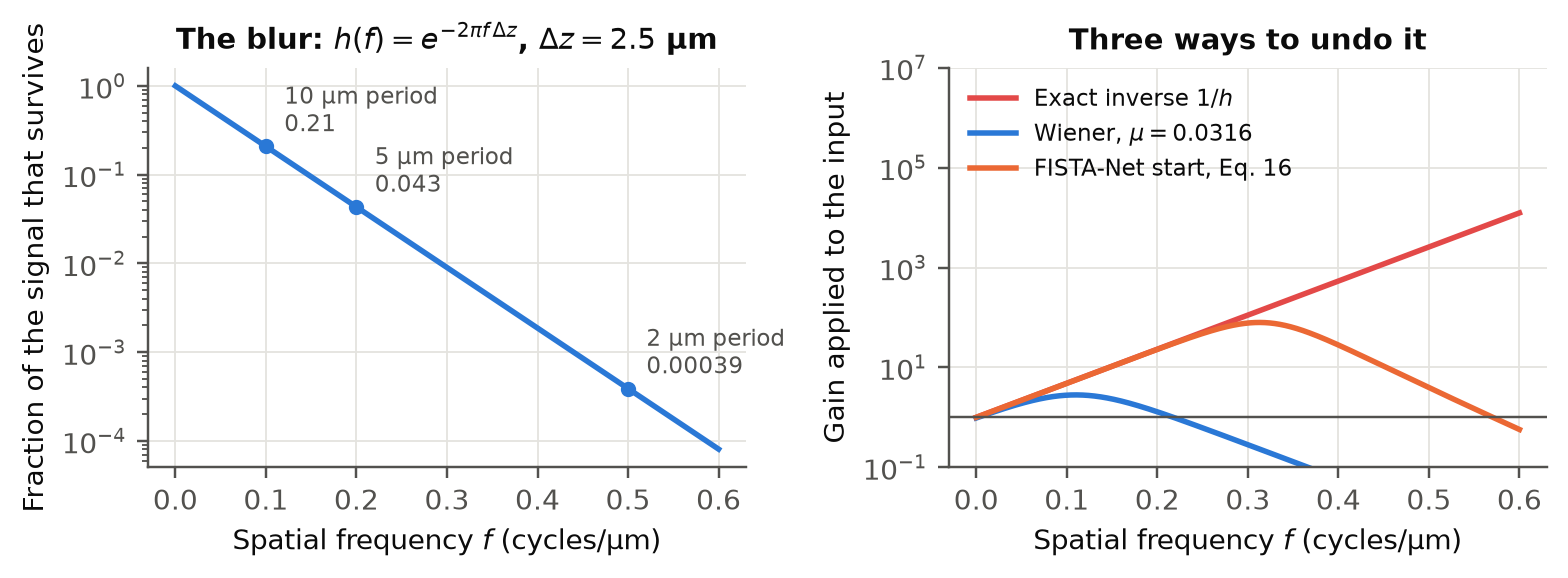
\includegraphics[width=\textwidth]{filters}
\caption{Left: how much of each frequency survives 2.5\um\ of standoff. Right: the gain three
methods apply to undo it. The red line is pure division. The blue and orange lines are the
Wiener filter and FISTA-Net's starting image, which you will meet in
Chapters~\ref{ch:classics} and~\ref{ch:fistanet}.}
\label{fig:filters}
\end{figure}

This kind of problem is called \textbf{ill-posed}. The measurement alone does not determine the
answer, so a method must add some extra belief about what fields look like. Every method in this
booklet differs mainly in what that extra belief is:

\begin{center}
\begin{tabular}{ll}
\toprule
Method & Extra belief \\
\midrule
Wiener & High frequencies are not worth trusting \\
ISTA, FISTA & The field is built from a few pieces of a dictionary \\
CSC-LISTA & Same, plus whatever training data teaches each layer \\
FISTA-Net & A small CNN learns what clean fields look like \\
\bottomrule
\end{tabular}
\end{center}

\section{How we score a result}\label{sec:score}

\textbf{Relative $L_2$ error} is the main number:
\begin{equation}
\text{error} = \frac{\lVert y - t \rVert_2}{\lVert t \rVert_2}.
\end{equation}
Here $y$ is our output and $t$ is the true field. An error of 0\% is perfect. If you output a
blank image, you score exactly 100\%. For scale, the blurry input itself scores about 77\% on the
crop shown in Figure~\ref{fig:reconstruction}.

\begin{code*}{train_csc_lista.py}
def relative_l2(output, target):
    dims = (-2, -1)
    return torch.linalg.vector_norm(output - target, dim=dims) / torch.linalg.vector_norm(target, dim=dims)
\end{code*}

\textbf{NRMSE} is the second number: the root mean square error divided by the range of the
target. It looks much smaller, about 2--4\%, because the range of these fields is large compared
with their typical value. It is the same quality of result on a friendlier scale, so never
compare an NRMSE with a relative $L_2$.

\section{The 15 test pairs}

Our test data is COMSOL, the finite-element simulation. There are five coil configurations:
\code{L1_C1}, \code{IC_4um}, \code{C1+C2}, \code{C1+C2+C3} and \code{C1+C2+C3+C4}. Each gives
three components at both heights, so $5\times3=15$ pairs. Each reported score is the mean over
these 15.

\begin{careful}[15 pairs are not 15 independent tests]
They contain only two wire shapes. C2, C3 and C4 are mirror copies of C1, and
\code{IC_2um} and \code{IC_4um} are the same coil. This is why the scores for different
configurations look almost identical. Say ``15 pairs from two wire shapes''.
\end{careful}

\section{The rule that protects the result}

\begin{keyidea}[COMSOL is the exam, not the homework]
Models train only on simulated data. Settings and checkpoints are picked only on simulated
validation data. COMSOL is read once, after training, to produce the final score.
\end{keyidea}

There is one honest exception, covered in Chapter~\ref{ch:results}. The generator's width range,
speckle level and wire families were designed by looking at these same COMSOL coils. No
reconstruction score leaked, but the data was designed with the exam in mind.
